\subsection{IBM Spectrum Scale - GPFS}

Bei IBM Spectrum Scale, ehemalig \ac{GPFS}, handelt es sich um ein System, dass den gleichzeitigen Zugriff auf ein oder mehrere Dateisysteme von verschiedenen Knoten ermöglicht. Diese können mithilfe von unterschiedlichsten Techniken den Zugriff zur Verfügung stellen (\ac{SAN}, \ac{NAS}, \ac{DAS}) und ermöglichen das Aufsetzen eines hochperformanten skalierbaren Netzwerk \parencite[S. 1]{ibm.2017}.

Neben einfachem Datenzugriff werden eine Vielzahl zusätzlicher Features geboten: Datei Duplizierung, Regel basiertes Speicher Management, Kommunikation und Zusammenschluss verschiedener Rechenzentren und diverse andere. Auf diese wird hier aber nur sehr grob eingegangen, da sie größtenteils unrelevant für die Arbeit sind und deren Umfang übersteigen würden.

\textbf{Hauptkomponenten und Funktionen}

Von jedem Knoten des Clusters kann gleichzeitig auf sämtliche Daten zugegriffen werden. Aufgrund der \gls{POSIX} Kompatibilität kann der Zugriff über Systemfunktionen (open, read, write) oder spezielle APIs erfolgen. Dies vereinfacht die Bedienung erheblich, da der Cluster für den einzelnen Rechner wie eine ``normale'' Festplatte erscheint. Auf jedem GPFS Knoten sind drei Hauptkomponenten installiert:

\begin{itemize}
	\item \textbf{GPFS Administration Kommandos} \\
	Eine Reihe von Skripts und Programmen, die Konfigurationen ändern und Operationen auslösen können. Ausgeführte Kommandos können beliebige Knoten betreffen und werden entsprechend weitergeleitet und auf entfernten Systemen ausgeführt.
	\item \textbf{GPFS Kernelerweiterung} \\
	Diese Erweiterung bietet ein Interface zum Betriebssystem und ermöglicht es, GPFS als natives Dateisystem zu registrieren. Hierdurch erscheint der gesamte Cluster für eine Applikation wie eine einzelne Festplatte. Der Kernel führt diese entweder lokal auf verfügbarem Speicher aus oder leitet sie mithilfe des GPFS-Dämonen zu anderen Geräten weiter.
	\item \textbf{GPFS Daemon} \\
	Aufgabe dieses multithreaded Programmes ist das Ausführen sämtlicher Schreib-, Lese- und Pufferaktionen. Er sorgt auch für die Datenkonsistenz des Gesamtsystems. Zusätzlich zu den I/O-Aktionen wird auch die Kommunikation mit anderen Knoten im System ausgeführt, um Konfigurationsänderungen, Wiederherstellung und parallele Updates durchzuführen.
	Ebenfalls enthalten ist die Network Shared Disk-Komponente, die Cluster-weite Benennung von und den Zugriff auf Speicher zur Verfügung stellt \parencite[S. 6]{ibm.2017}.  
\end{itemize} 

\textbf{Clusterarten}

Es kann eine Vielzahl von Cluster Konfigurationen erreicht werden, da IBM Spectrum Scale unterschiedlichste Betriebssysteme unterstützt (speziell Linux, AIX, Windows) und Speicher auf verschiedene Arten anschließbar ist. Im Folgenden werden zwei häufig verwendete Szenarien vorgestellt.

Eine Variante ist der Anschluss von sämtlichen Knoten an das selbe Storage Area Network. Ist dies nicht der Fall, können nur einzelne Nodes als \ac{NSD} Server angeschlossen sein und die verbleibenden sind \ac{NSD} Klienten. Hierbei wird eine klassische Server-Client Architektur aufgesetzt bei der eine Vielzahl von GPFS Klienten auf eine kleinere Anzahl von GPFS Servern mit Speicheranbindung zugreift \parencite[S. 8]{ibm.2017}. Dies ist in \autoref{fig:gpfsarchitecture} verdeutlicht.

\begin{figure}[hbt]
	\centering
	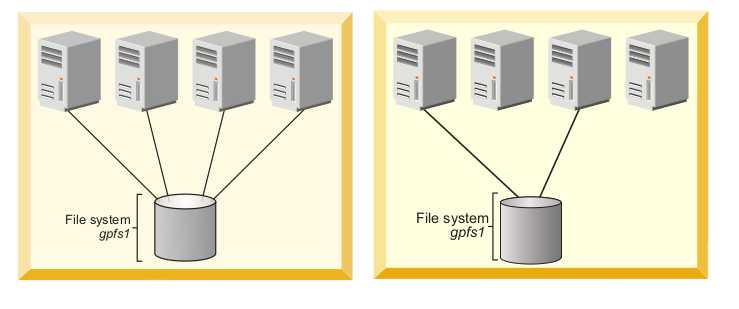
\includegraphics[scale=0.6]{images/gpfs-architectures}
	\caption{Anbindung an alle Knoten (links) und Server-Klient Architektur (rechts) \parencite[S. 8]{ibm.2017}}
	\label{fig:gpfsarchitecture}
\end{figure}

\textbf{Verbindung mit Cloud-Diensten}

IBM Spectrum Scale unterstützt aktuell zwei Cloudfunktionen: \textbf{Cloud Tiering} und \textbf{Data Sharing}. Es können maximal vier verschiedene Knoten und ein Dateisystem für diese Dienste verwendet werden \parencite{mani.2017}.

Im ersten Szenario - dem sogenannten Cloud Tiering - werden so genannte kalte Daten (also Dateien, die selten benutzt werden und geringe Zugriffsraten erfordern) in der Cloud gespeichert, um die schnellen lokalen Datenspeicher zu entlasten. Dadurch kann die Clusterperformance erhöht und Kosten für zusätzlichen lokalen Speicher gespart werden. Diese Funktion ist in das \ac{ILM} System eingebunden und ermöglicht es den Administratoren Strategien zu definieren, um die Auslagerung bei bestimmten Daten auszulösen.
Es sollten nur kalte Files in der Cloud gespeichert werden, da diese bei Zugriff herunterzuladen sind, was die Latenz massiv erhöht \parencite[S. 107]{ibm.2017}.
Lokal wird ein Cloudverzeichnis angelegt, welches alle migrierten Daten auflistet. Bei diesem Verzeichnis handelt es sich um einen speziellen Ordner in einem Filesystem von Spectrum Scale, welches mit dem entsprechenden Cloudaccount verbunden ist. Wird auf einen sogenannten Datei-Stub (eine Art Referenz auf die Datei) zugegriffen, kann die ferne Information heruntergeladen werden. In der Cloud liegen pro File zwei verschlüsselte Dateien, eine für die eigentlichen Daten und eine zweite mit Metadaten (Besitzer, Zugriffsrechte, u.a.) \parencite[S. 108]{ibm.2017}.

Cloud Data Sharing ermöglicht das Teilen von lokalen Daten mit verschiedenen Arten von Objektspeichern (siehe \autoref{subsec:objectstorage}). Dieser Export kann ebenfalls durch \ac{ILM} Strategien in regelmäßigen Zyklen ausgelöst werden, um zum Beispiel Daten in der Cloud aktuell zu halten. Diese können dann von anderen Applikationen verwendet werden. Es ist ebenfalls ein Import vom Object Storage System möglich, um die lokalen Daten gegebenenfalls zu erweitern.
Der Export wird parallel mit allen Clouddienstknoten durchgeführt. Dabei kann eine Liste aller Daten in einem Manifest gespeichert werden, um diese später nachzuverfolgen.\\
Der größte Unterschied zur Migration beim Cloud Tiering ist, dass die Dateien in der Cloud nicht verschlüsselt werden, da sie auch für andere Nutzer verfügbar sein sollen und dass nach einem Transfer keine Verbindung (d.h. keine Updates bei späteren Änderungen) mehr zwischen lokalen und entfernten Files besteht \parencite[S. 109]{ibm.2017}.

Konfiguration dieser beiden Funktionalitäten kann mit dem \lstinline|mmcloudgateway| Programm vorgenommen werden \parencite{scale.2017}.

\subsection{Apache Hadoop - HDFS}

Apache Hadoop (ab hier nur noch Hadoop) ist ein Framework zur Entwicklung von massiven verteilten Systemen. Es ist in der Lage, große Mengen von Daten sowohl strukturiert als auch unstrukturiert, über viele verteilte Berechnungsknoten zu verteilen und zu bearbeiten. Das Hauptsystem von Hadoop verwendet ein eigenes Dateisystem: \ac{HDFS} \parencite[Kap. I,1]{alapati.2016}.

Dieses System sorgt für eine automatische Datenreplikation und unterstützt ebenfalls das leichte Hinzufügen von weiteren Servern mit zusätzlichem Plattenspeicher. Ein typischer Hadoop Cluster besteht aus Master- (hier läuft die Hadoop-Software), Arbeiterknoten (zur Bereitstellung von Speicher mit \ac{HDFS} und Rechenleistung mit \ac{YARN}) und so genannten Edge-Servern (Zugriff auf den Cluster zum Ausführen von Programmen). Zusätzlich kann es noch Server für weitere Frameworks geben und Datenbanken für spezielle Metadaten \parencite[Kap. I,1]{alapati.2016}.

Die Bearbeitung der Daten kann mithilfe verschiedener Anwendungsframeworks passieren, besonders beliebt ist hierbei MapReduce und Apache Spark.

Standardmäßig repliziert HDFS jeden Datensatz dreimal, um eine hohe Ausfallsicherheit zu garantieren. Es wird ein \ac{WORM} Zugriffsmodel verwendet, sodass Konsistenz kein Problem darstellt, da immer nur ein Nutzer auf eine Datei schreiben kann. Daten werden in große Blöcke (zum Beispiel 256 MB) aufgeteilt und auf verschiedenen Maschinen gespeichert. Hierdurch können auch sehr große Files gesichert werden, die für einzelne Maschinen zu viel Speicher brauchen würden. Metadaten für alle Blöcke werden innerhalb einer NameNode im RAM und auf konsistentem Speicher gesichert  \parencite[Kap. I,2]{alapati.2016}.

Hadoop kann auch komplett in der Cloud verwendet werden. Es gibt einige Hosting-Anbieter (Amazon EC2, Google Computing Engine), die einen dynamischen Funktionsumfang zur Verfügung stellen \parencite[Kap. I, 1]{alapati.2016}.

\subsection{Objektdateisysteme} \label{subsec:objectstorage}

Objektspeicher ist eine moderne Speichertechnologie und eine logische Weiterentwicklung von Block- oder Dateispeichern. Er virtualisiert die physische Implementierung komplett von der logischen Darstellung. Als Nutzer übergibt man seine Daten in das System, weiß aber nicht, wo diese dann genau gespeichert werden. Es soll Probleme von klassischen Lösungen wie komplexe Speicherhierachie, Fragmentierung von Filesystemen, sowie Komplexität von Sicherheit und Zugriffsoperationen umgehen \parencite[Kap. 1, Object Storage]{varma.2015}.

\begin{figure}[hbt]
	\centering
	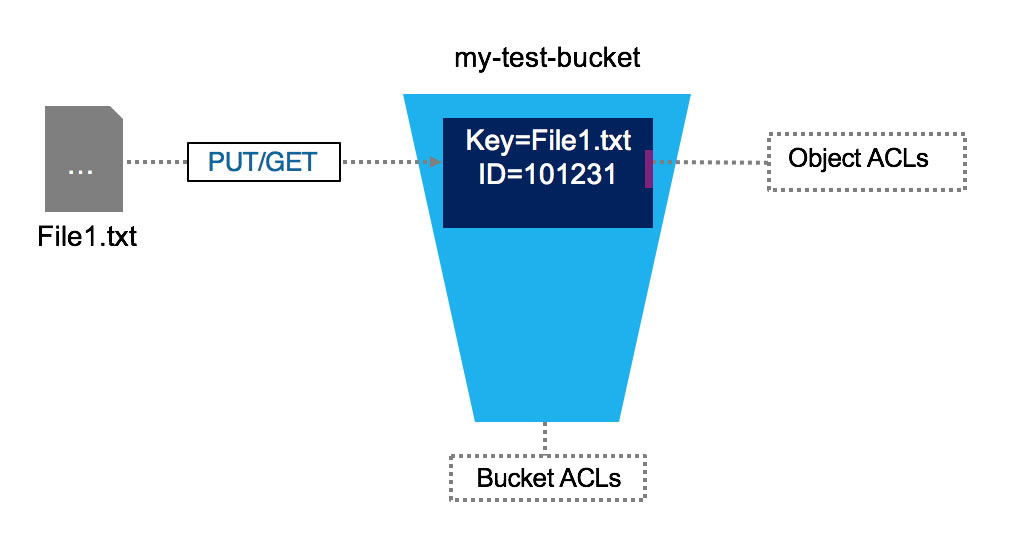
\includegraphics[scale=0.4]{images/object-storage}
	\caption{Komponenten von Objektspeichern \parencite[S. 5]{Rios.2017}}
	\label{fig:objectstorage}
\end{figure}

Dieser Typ von Dateisystem umfasst drei Hauptkomponenten:

\begin{itemize}
	\item \textbf{Daten:}\\
	 Nutzer und Anwendungsinformationen, die persistent hinterlegt werden müssen. Jede Art von Format ist hierbei unterstützt.
	\item \textbf{Metadaten:}\\
	 Diese sind Informationen über die eigentlichen Daten wie zum Beispiel Dateigröße oder Uploadzeitpunkt. Ebenfalls können benutzerdefiniert Schlüssel-Wert Paare von nutzenden Anwendungen gespeichert werden. Diese sind von den Applikationen oder Usern zu jeder Zeit frei veränderbar. Eine Besonderheit dieses Filesystems ist, dass die Metadaten zusammen mit den eigentlichen Daten gespeichert werden.
	\item \textbf{\ac{UUID}:} Diese eindeutige ID wird jedem Objekt im Speicher zugeordnet. Mit ihr können Daten unterschieden  und gefunden werden, unabhängig von der physikalischen Position der eigentlichen Informationen.
\end{itemize}

Durch obige Eigenschaften wird eine flache Hierarchie erzeugt, die Probleme mit außer Kontrolle geratenen Metadatenspeichern verhindert. Daten können in sogenannten Buckets zusammengefasst werden, um eine logische Strukturierung einzuführen und gegebenenfalls die Zugriffsrechte von Nutzern einschränken zu können.  

Da diese Art von Daten fast immer in der Cloud oder auf einem entfernen Server gespeichert werden, bieten sich besonders REST-Schnittstellen zum Zugriff auf die Daten an \parencite[S. 4f]{Rios.2017}.

Objektspeicher sind dafür ausgelegt gut zu skalieren, das heißt es kann unterschiedliche Hardware mit kompletten Dateisystemen zusammengeschlossen werden. Die wichtigste Aufgabe wird hierdurch die richtige Platzierung von Daten und die Automatisierung von Management Aufgaben, um die Stabilität zu erhöhen \parencite[Kap. 1, Object Storage]{varma.2015}.
